This section outlines the initial approach to solve the functions shown in the functional block diagram. The functional block diagram of the project can be found in Figure \ref{fig:Func} in Part 3 of this document.

The core of the functional block diagram is the processing unit which is implemented in the form of a 32 bit microcontroller with an algorithm embedded in firmware. The microcontroller that will be implemented in the final design will be determined by the amount digital inputs and outputs (IO) required as well as the amount of mathematical equations required per second.

The microcontroller will act on instructions received through a wireless communication channel that originate from a smartphone application. The application will only act as a user interface for the robot and will output basic instructions for the robot to follow.

\subsubsection{Design alternatives}
The two wireless technologies built into most modern smartphones that best suit the needs of the communication channel is Wi-Fi and Bluetooth. Journal article \cite{Dhawan:Analogy} makes some comparisons between these two similar but different technologies. Wi-Fi has a much higher bandwidth than Bluetooth as well as far superior range. Wi-Fi networks are generally much more complex than Bluetooth networks. Bluetooth is also better suited for peer to peer communication whereas Wi-Fi is mostly intended to be used with a router. Network security for Wi-Fi is much more advanced and therefore much more secure than that of Bluetooth.

After the commands are passed from the smartphone to the microcontroller, the microcontroller interfaces to actuators to execute the movements desired by the user. When considering possible actuators that can be used, thee possible solutions come to mind. These are servo motors, geared DC motors and stepper motors. Geared DC motors are small, light and easy to implement but lack feedback on shaft position. Such feedback needs to be implemented manually to be able to make controlled movements. Stepper motors have fixed step resolution so making controlled movements is easier once the current position is known. The drawback of these motors is that a homing mechanism and routine needs to be implemented to find a reference. Stepper motors are also heavy and require high current even when stationary. Servo motors are basically geared DC motors with a positional feedback control system built-in. The motor only receives power and a desired position and it will attempt to reach the position. The disadvantage is that these have a limited range of motion.

The overall shape of the robot and, more specifically, the placement of legs around the robot will greatly influence the robot's performance when moving forward in a straight line, moving sideways and moving over obstacles.

A popular design in hexapod robots is placing the legs in groups of three on opposite sides. This means that the legs are all aligned in a similar direction while the body is usually a long rectangular shape, similar to that found on insects. The advantage of this design lies mainly in the ability to move forward very quickly since the legs are placed optimally for forward motion. While holonomic movement is possible, it is usually much slower than forward or backward motion. This design is usually more suited to robots with an even number of legs due to the symmetry of the design.

An alternative design approach is to space the legs evenly around the robot chassis. The robot chassis would normally be round or a polygon with the same number of sides as legs. In the case of a five legged robot, the legs would be positioned $\frac{360^o}{5} = 72^o $ apart.
This equally spaced design approach has the disadvantage of not being particularly fast in any given direction but the advantage that it can manage the maximum speed in any given direction. Figure \ref{fig:Body_layout} shows an examples of both layouts.
\begin{figure*}[t!]
    \centering
    \begin{subfigure}[t]{0.5\textwidth}
        \centering
        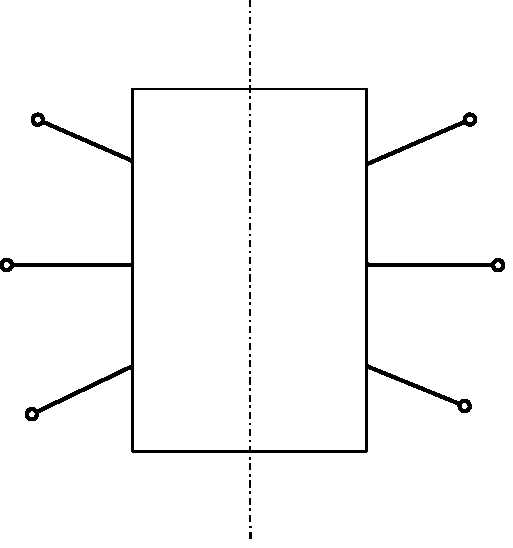
\includegraphics[scale = 0.6]{pics/Body_layout_hex.pdf}
        \caption{Symmetric chassis layout.}
    \end{subfigure}%
    ~ 
    \begin{subfigure}[t]{0.5\textwidth}
        \centering
        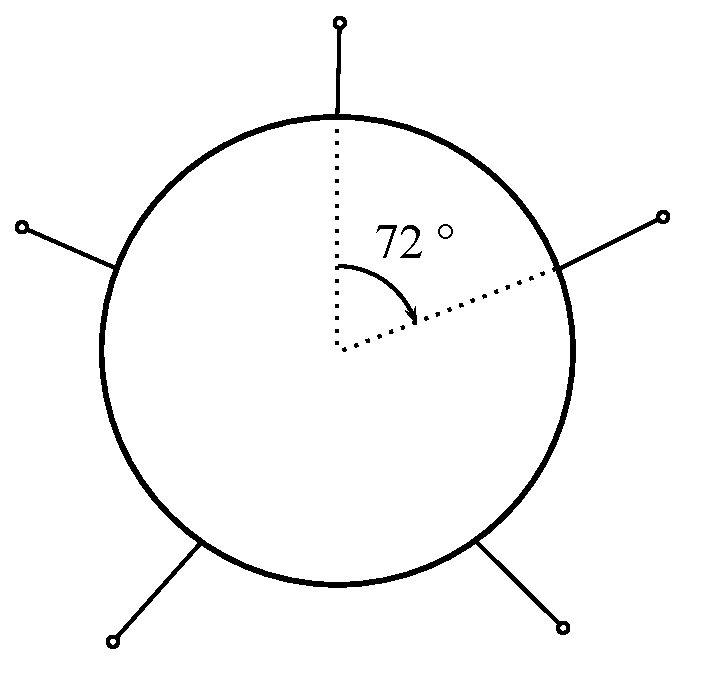
\includegraphics[scale = 0.5]{pics/Body_Layout.pdf}
        \caption{Equally spaced chassis layout.}
    \end{subfigure}Example of an e
    \caption{Examples of two different chassis layout options for legged robots.}
    \label{fig:Body_layout}
\end{figure*}

\subsubsection{Preferred solution}
Since the data transfer in the communication channel between the smartphone and the robot consists only of simple commands and the required bandwidth is therefore low, Bluetooth will be used instead of Wi-Fi. Bluetooth has the advantage of being less expensive and far less complicated to implement. The added security that Wi-Fi offers is not required for this application. The disadvantage of using Bluetooth instead of Wi-Fi is the very limited range that Bluetooth offers.\\

The commands received via Bluetooth will be actuated with the use of servo motors. These compact units are ideal for this scenario as they have all of the advantages of geared DC motors with all of the required control systems built-in. Servo motors have the advantage that they are usually light for the torque they can provide, which is ideal for a robot where weight is often a problem.\\

This will all be implemented in a circular shaped chassis with equally spaced legs as this design is better suited for holonomic movements than the symmetric design.

